\documentclass[10pt,landscape,a4paper,twocolumn]{article}
\usepackage{kotex}
\usepackage{graphicx}
\graphicspath{ {./images/} }

\setlength{\columnsep}{20pt}

\usepackage[left=1.0cm, right=1.0cm, top=1.5cm, bottom=0.6cm, headsep=0.4cm]{geometry}
\usepackage{amsmath}
\usepackage{amssymb}
\usepackage{fontspec}
\usepackage{kotex}
\usepackage{graphicx}
\usepackage{setspace}
\usepackage{listings}
\usepackage{comment}
\usepackage{import}
\usepackage{wrapfig}
\usepackage{url}
\usepackage{array}
\usepackage[normal]{engord}
\usepackage[svgnames,table]{xcolor}


\usepackage{fancyhdr}
\pagestyle{fancy}
\fancyhead[R]{\thepage}
\fancyhead[L]{Seoul National University - Another LEVEL}
\setmonofont{SourceCodePro-Regular.ttf}
\setmainhangulfont{NanumMyeongjo}
\setlength\parindent{0pt}
\usepackage[parfill]{parskip}

\definecolor{dkgrey}{RGB}{127, 127, 127}

\lstset{basicstyle=\footnotesize\ttfamily,
    breaklines=true,
    breakindent=1.1em,
%   numbers=left,
%   numberstyle=\footnotesize\ttfamily\color{dkgrey},
%   numbersep=5pt
%   frame=trbl
}

\lstdefinestyle{mycpp}{
    language=[GNU]C++,
    keywordstyle=\color{blue},
    commentstyle=\itshape\color{purple!40!black},
    stringstyle=\color{orange},
}


\begin{document}
\tableofcontents

\section{Setting}
\subsection{Header}
\lstinputlisting{src/Setting/Header.cpp}

\subsection{vimrc}
\lstinputlisting{src/Setting/vimrc}

\subsection{Sublime text}
\lstinputlisting{src/Setting/mycpp.sublime-build}

\section{String}
\subsection{KMP}
\lstinputlisting{src/String/KMP.cpp}

\subsection{Aho Chorasick}
\lstinputlisting{src/String/AhoChorasick.cpp}

\subsection{Suffix array}
\lstinputlisting{src/String/SuffixArray.cpp}

\subsection{Manacher's algorithm}
\lstinputlisting{src/String/Manacher.cpp}

\subsection{Z algorithm}
\lstinputlisting{src/String/ZAlgorithm.cpp}


\section{Graph \& Flow}
\subsection{BCC}
\lstinputlisting{src/Graph/BCC.cpp}

\subsection{Hopcroft Karp}
\lstinputlisting{src/Graph/HopcroftKarp.cpp}

\subsection{Dinic}
\lstinputlisting{src/Graph/Dinic.cpp}

\subsection{MCMF}
\lstinputlisting{src/Graph/MCMF.cpp}

\subsection{Blossom}
\lstinputlisting{src/Graph/Blossom.cpp}

\subsection{Stoer Wagner}
\lstinputlisting{src/Graph/Stoer_Wagner.cpp}

\subsection{Dominator Tree}
\lstinputlisting{src/Graph/DominatorTree.cpp}

\subsection{LR-flow}
\lstinputlisting{src/Graph/LRflow.cpp}

%\lstinputlisting{}
\section{Query}

\subsection{Splay Tree2}
\lstinputlisting{src/Query/splay2.cpp}

\subsection{Link Cut Tree}
\lstinputlisting{src/Query/LinkCut.cpp}

\subsection{HLD}
\lstinputlisting{src/Query/HLD.cpp}

\subsection{Mo Hilbert Order}
\lstinputlisting{src/Query/MoHilbertOrder.cpp}

\subsection{Lazy Propagation 1}
\lstinputlisting{src/Query/Lazy1.cpp}

\subsection{Dynamic Convex Hull Trick}
\lstinputlisting{src/Query/DynamicConvexHullTrick.cpp}


\section{Geometry}

\subsection {Voronoi}
\lstinputlisting{src/Geometry/Voronoi.cpp}

\section{Math}
\subsection{FFT}
\lstinputlisting{src/Math/fft.cpp}

\subsection{Kirchhoff Theorem}
\lstinputlisting{src/Math/Kirchhoff.txt}

\subsection{Berlekamp Massey}
\lstinputlisting{src/Math/Berlekamp_Massey.cpp}

\subsection{Simplex}
\lstinputlisting{src/Math/simplex.cpp}

\subsection{Gaussian Elimination}
\lstinputlisting{src/Math/GaussianElimination.cpp}

\subsection{Prime Algorithms}
\lstinputlisting{src/Math/PrimeAlgorithms.cpp}


\section{Miscelleneous}

\subsection{Hungarian}
\lstinputlisting{src/Miscelleneous/Hungarian.cpp}

\subsection{LiChao Tree}
\lstinputlisting{src/Miscelleneous/LiChaoTree.cpp}

\subsection{Persistence Segment Tree}
\lstinputlisting{src/Miscelleneous/PersistenceSegTree.cpp}

\subsection{Various FFTs (Bitwise Convolution)}
\lstinputlisting{src/Miscelleneous/BitwiseConvolution.cpp}

\subsection{NTT}
\lstinputlisting{src/Miscelleneous/NTT.cpp}

\subsection{Order Statistic Tree}
\lstinputlisting{src/Miscelleneous/OrderStatisticTree.cpp}

\subsection{BITSET}
\lstinputlisting{src/Miscelleneous/BITSET.cpp}

\subsection{Bit Hacks}
\lstinputlisting{src/Miscelleneous/BitHacks.cpp}

\subsection{Fast IO}
\lstinputlisting{src/Miscelleneous/fastio.cpp}

\begin{figure}[ht]
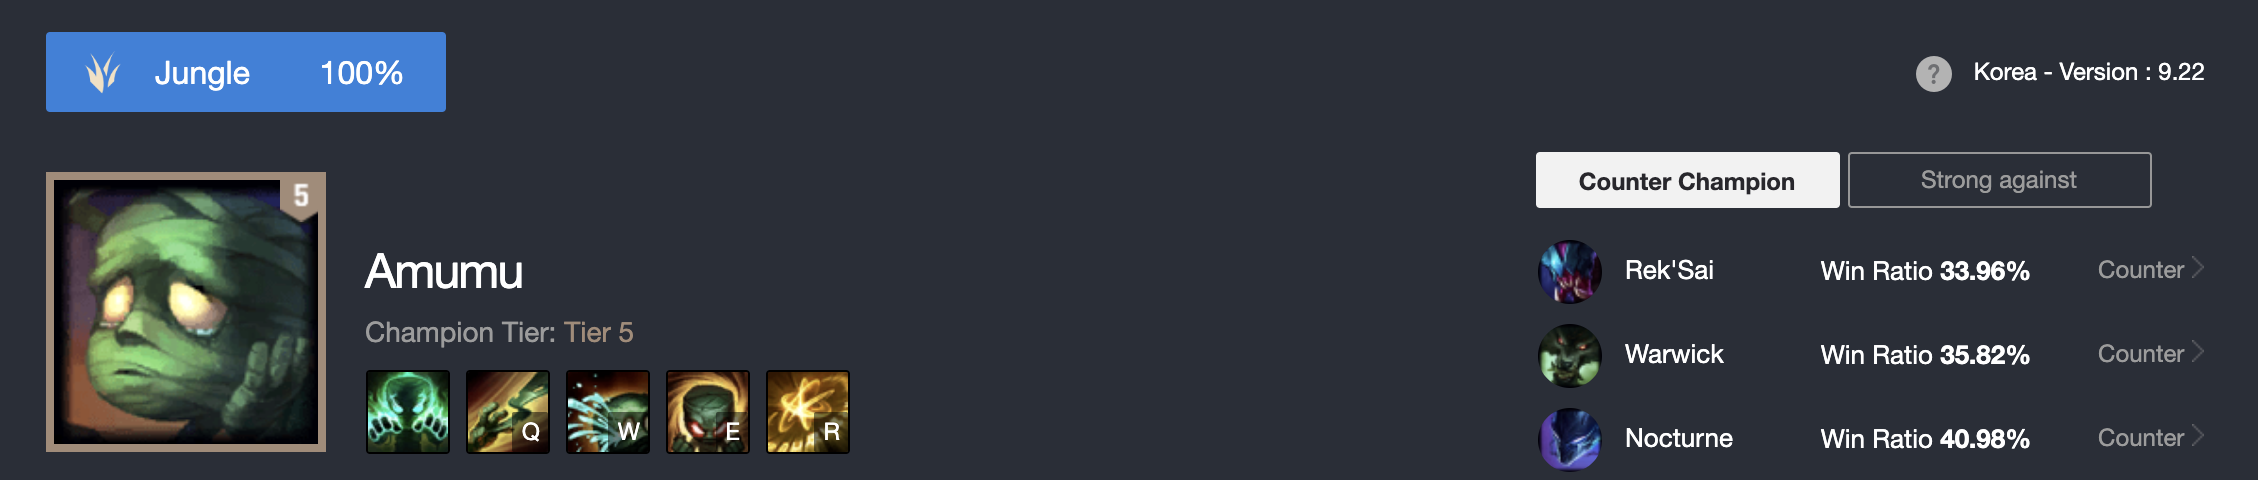
\includegraphics[scale=0.3]{1}
\end{figure}
\begin{figure}[ht]
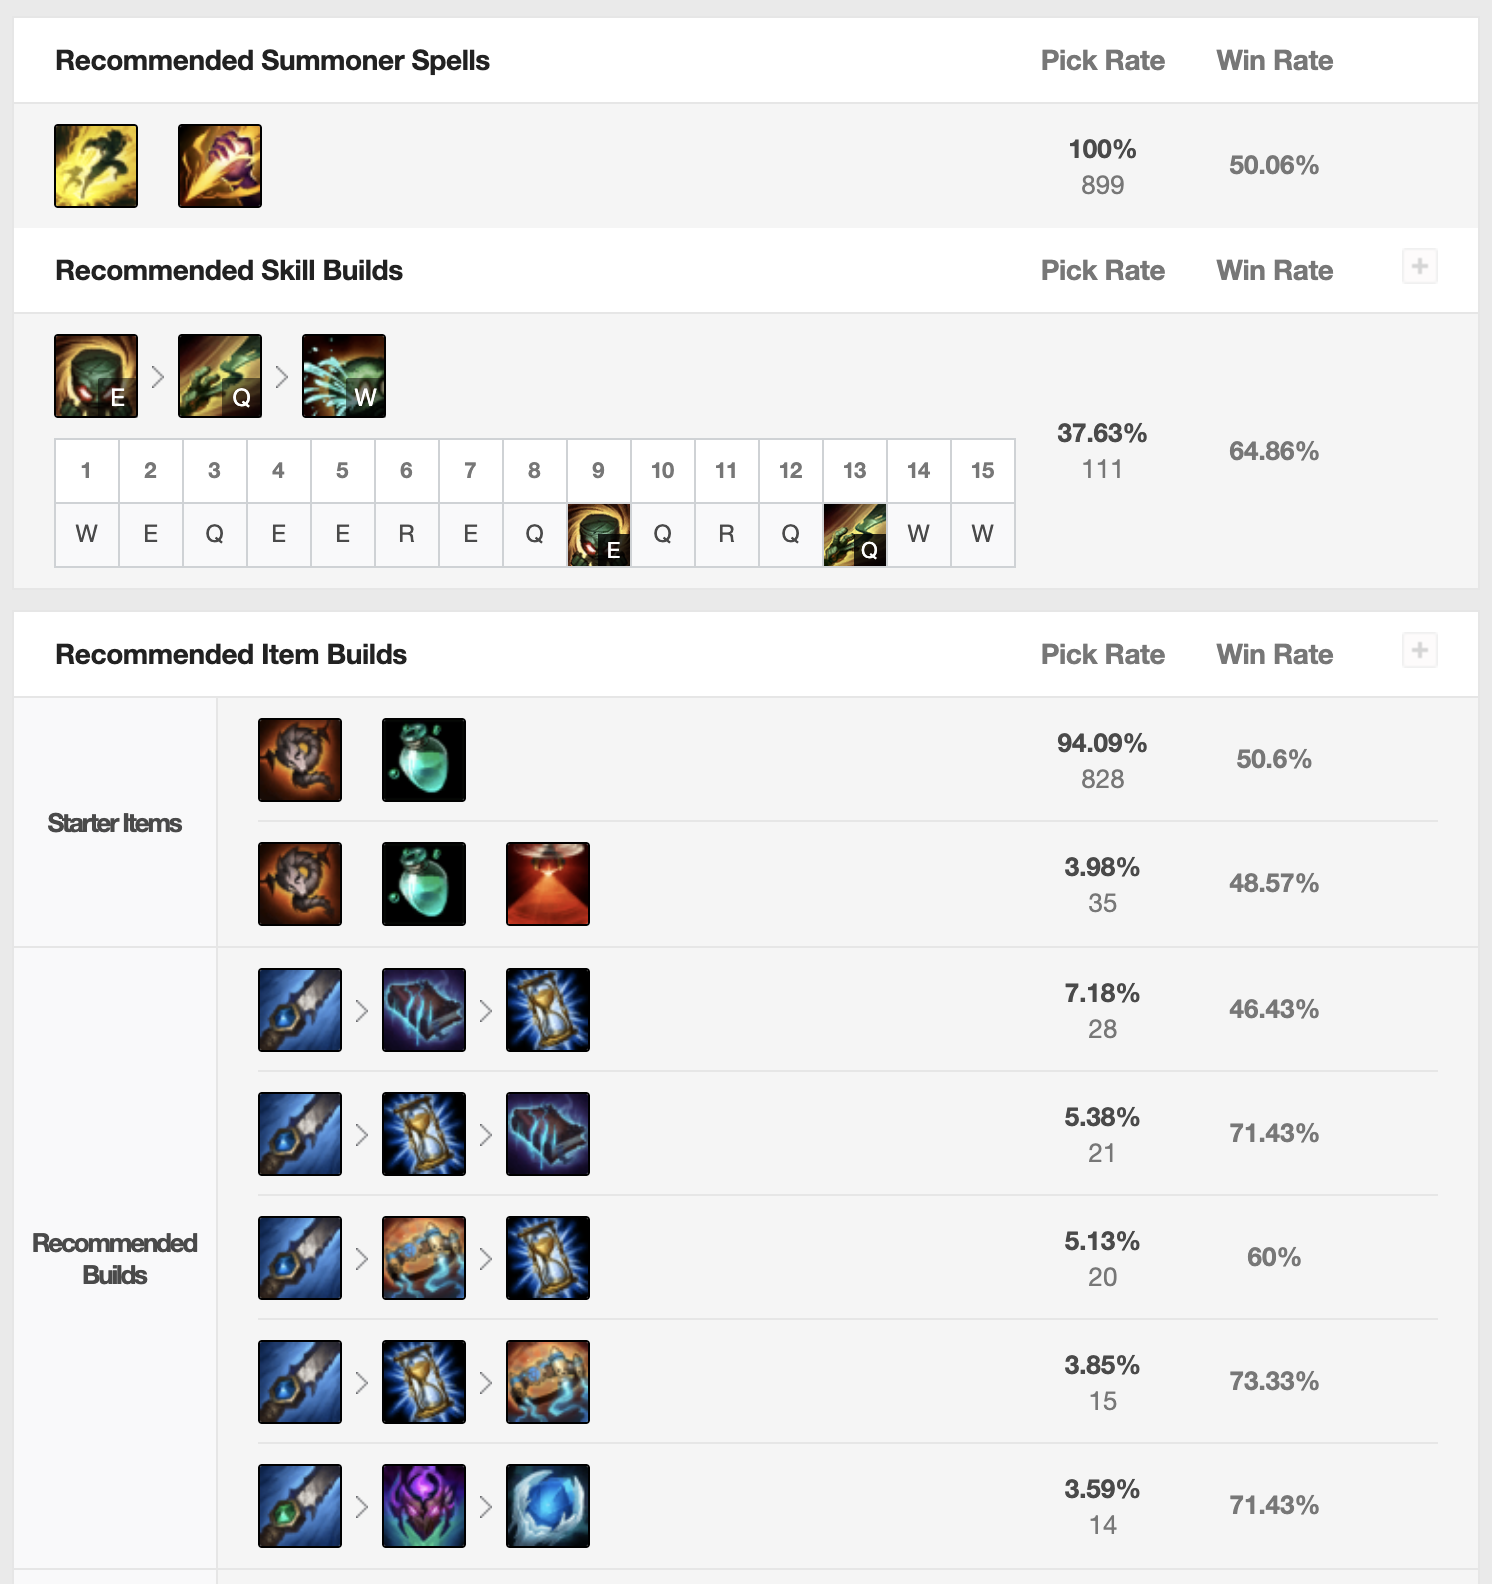
\includegraphics[scale=0.3]{2}
\end{figure}
\begin{figure}[ht]
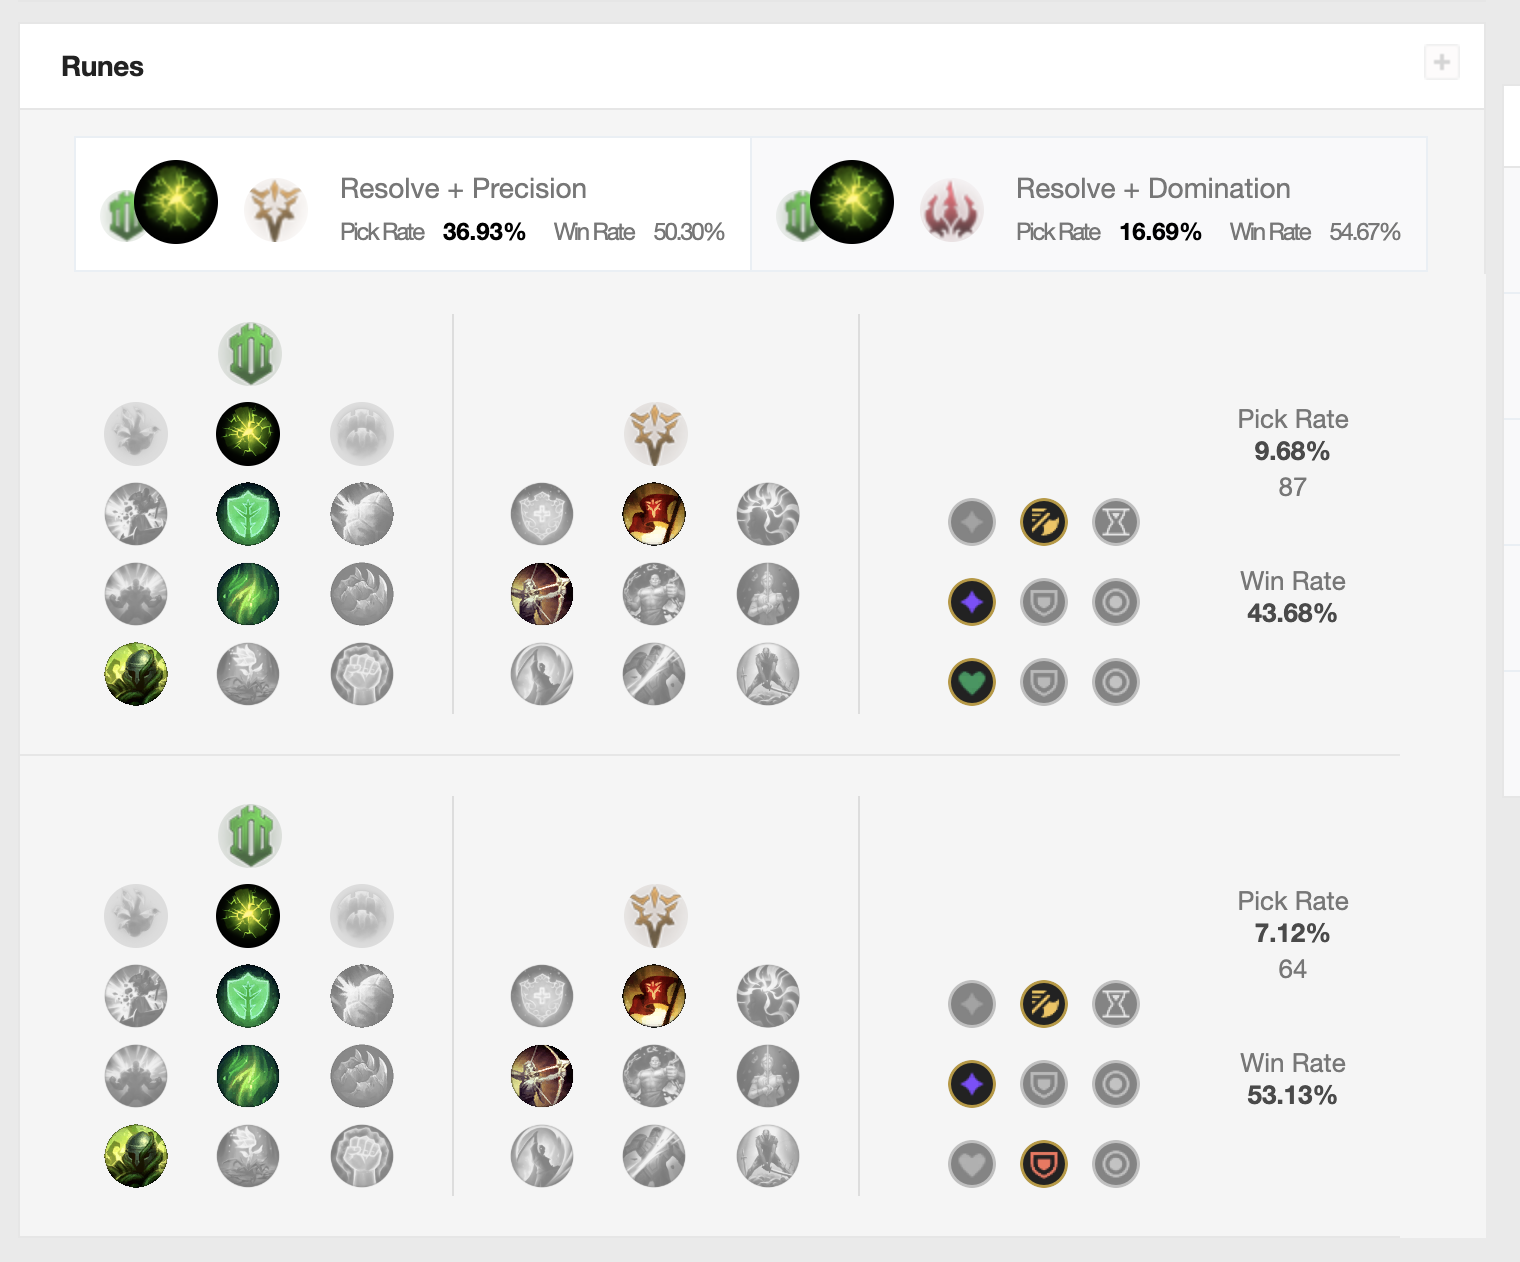
\includegraphics[scale=0.3]{3}
\end{figure}

\begin{figure}[ht]
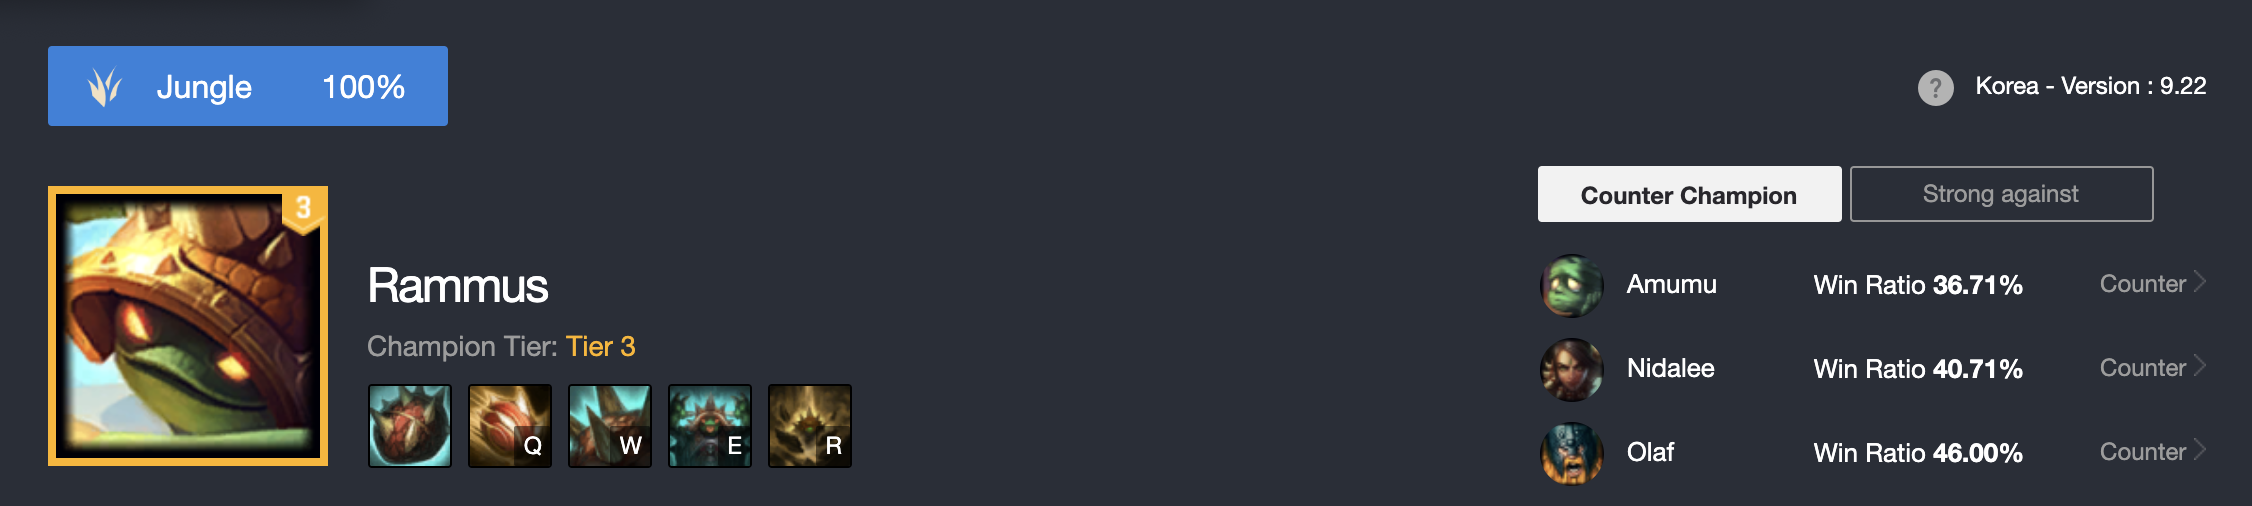
\includegraphics[scale=0.3]{4}
\end{figure}
\begin{figure}[ht]
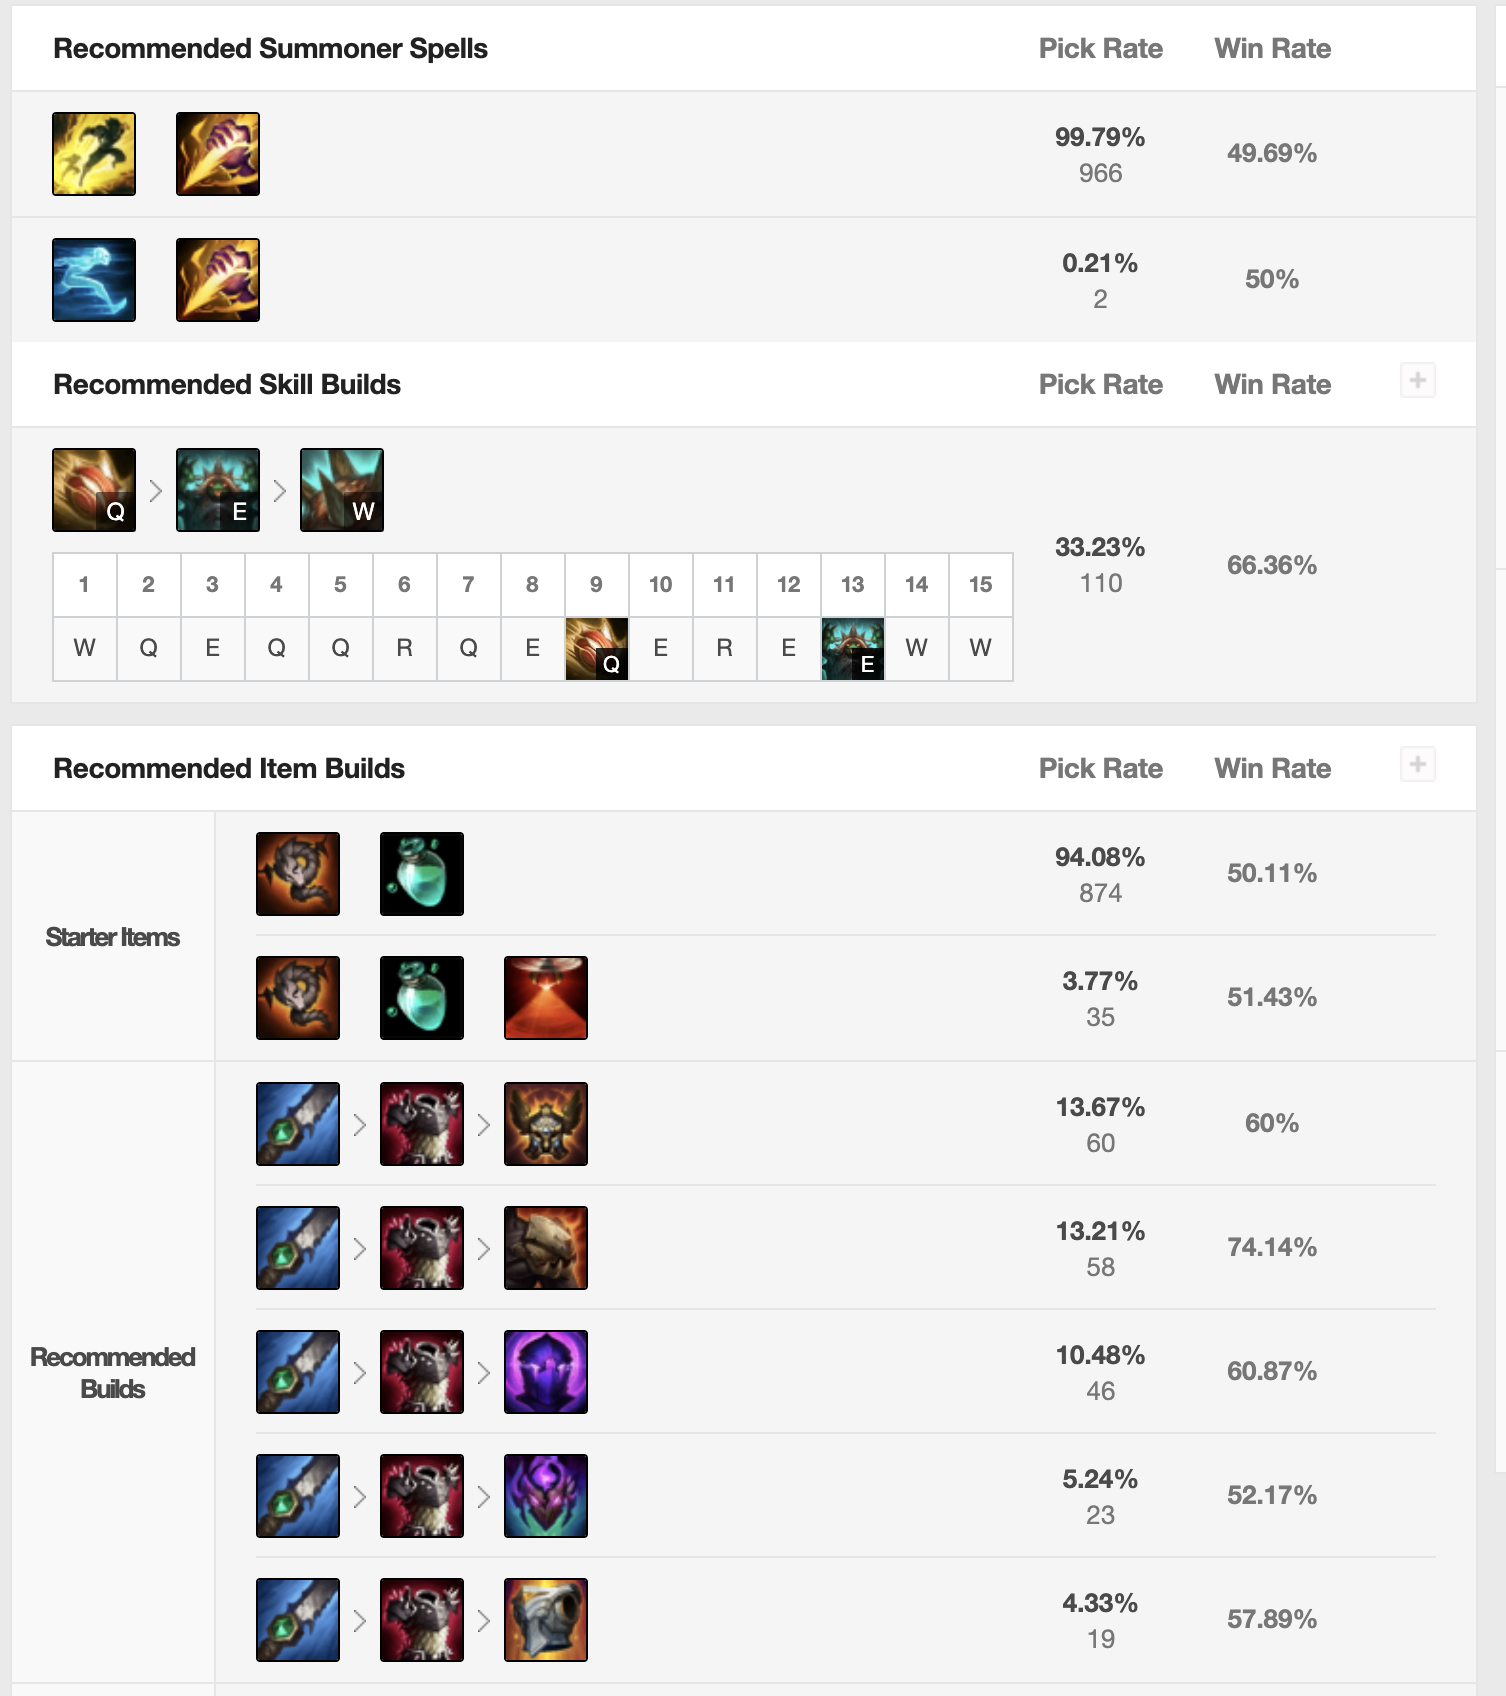
\includegraphics[scale=0.3]{5}
\end{figure}
\begin{figure}[ht]
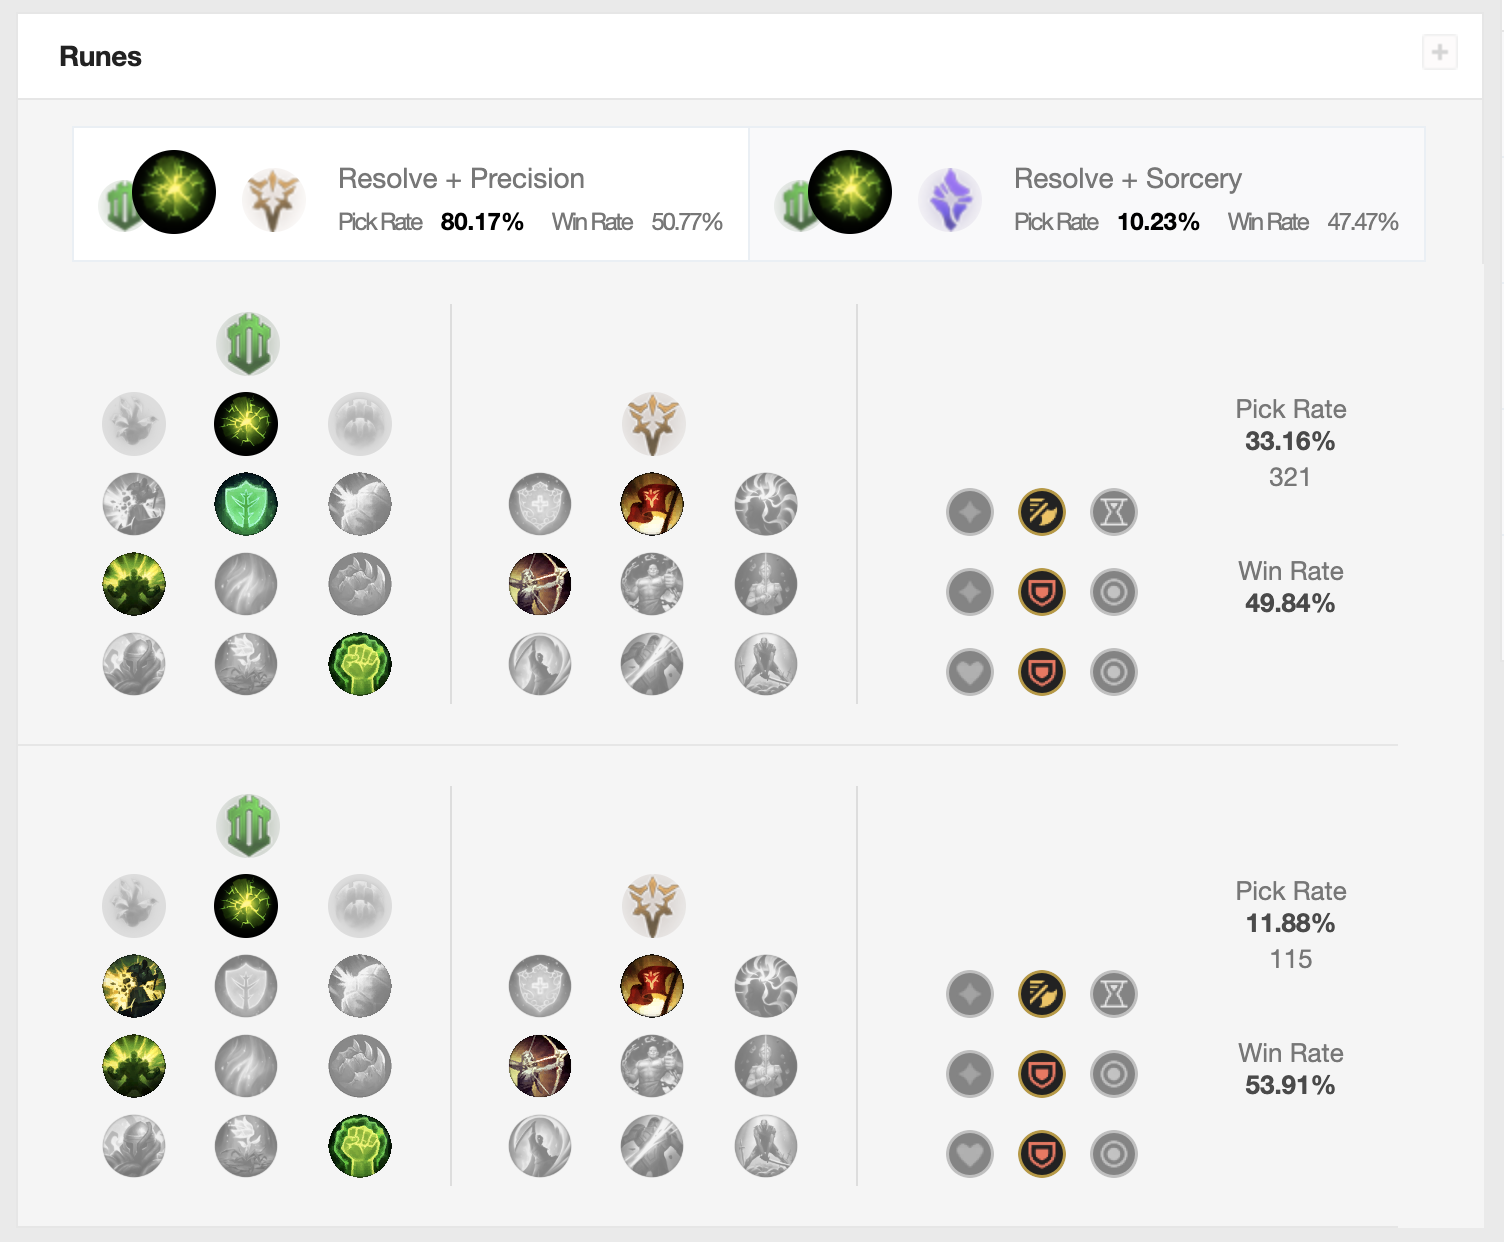
\includegraphics[scale=0.3]{6}
\end{figure}

\begin{figure}[ht]
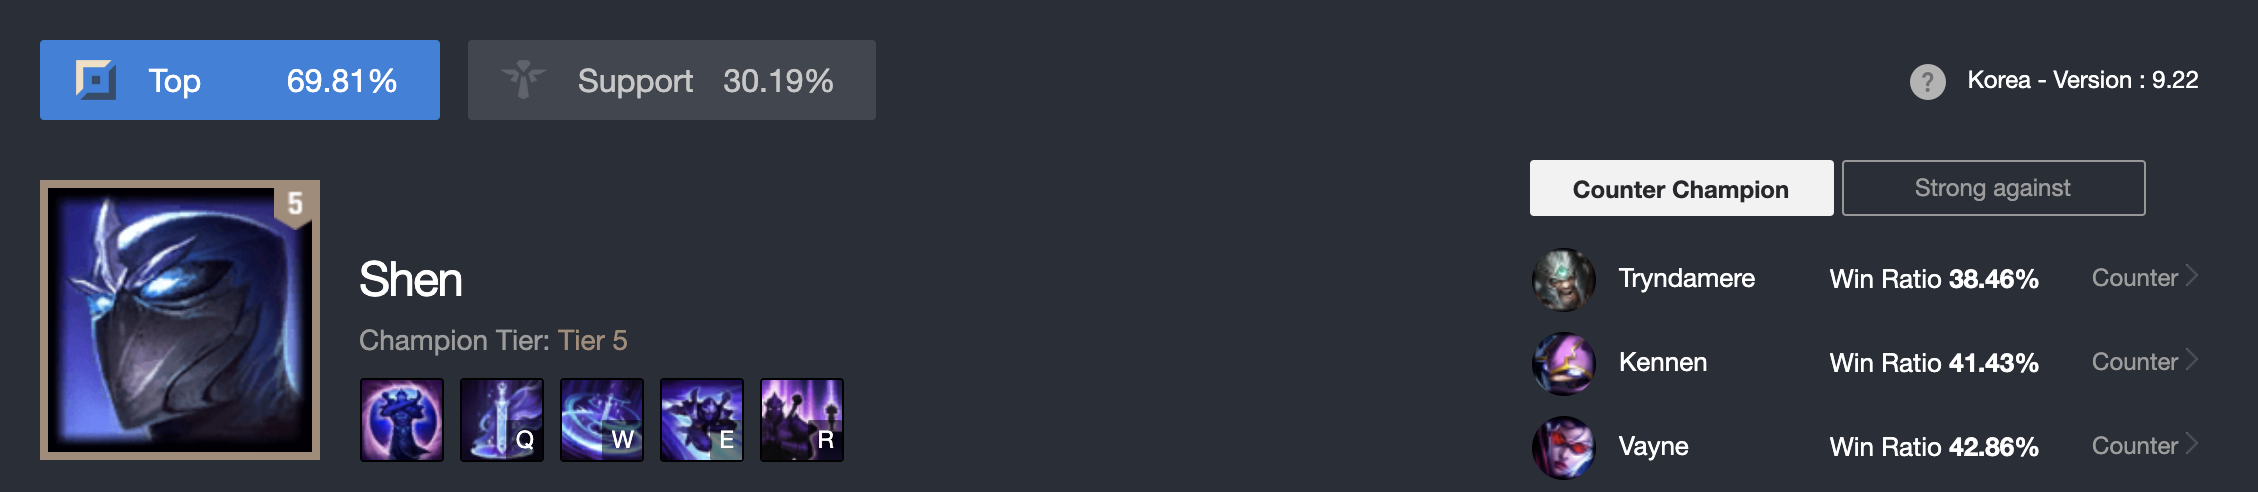
\includegraphics[scale=0.3]{7}
\end{figure}
\begin{figure}[ht]
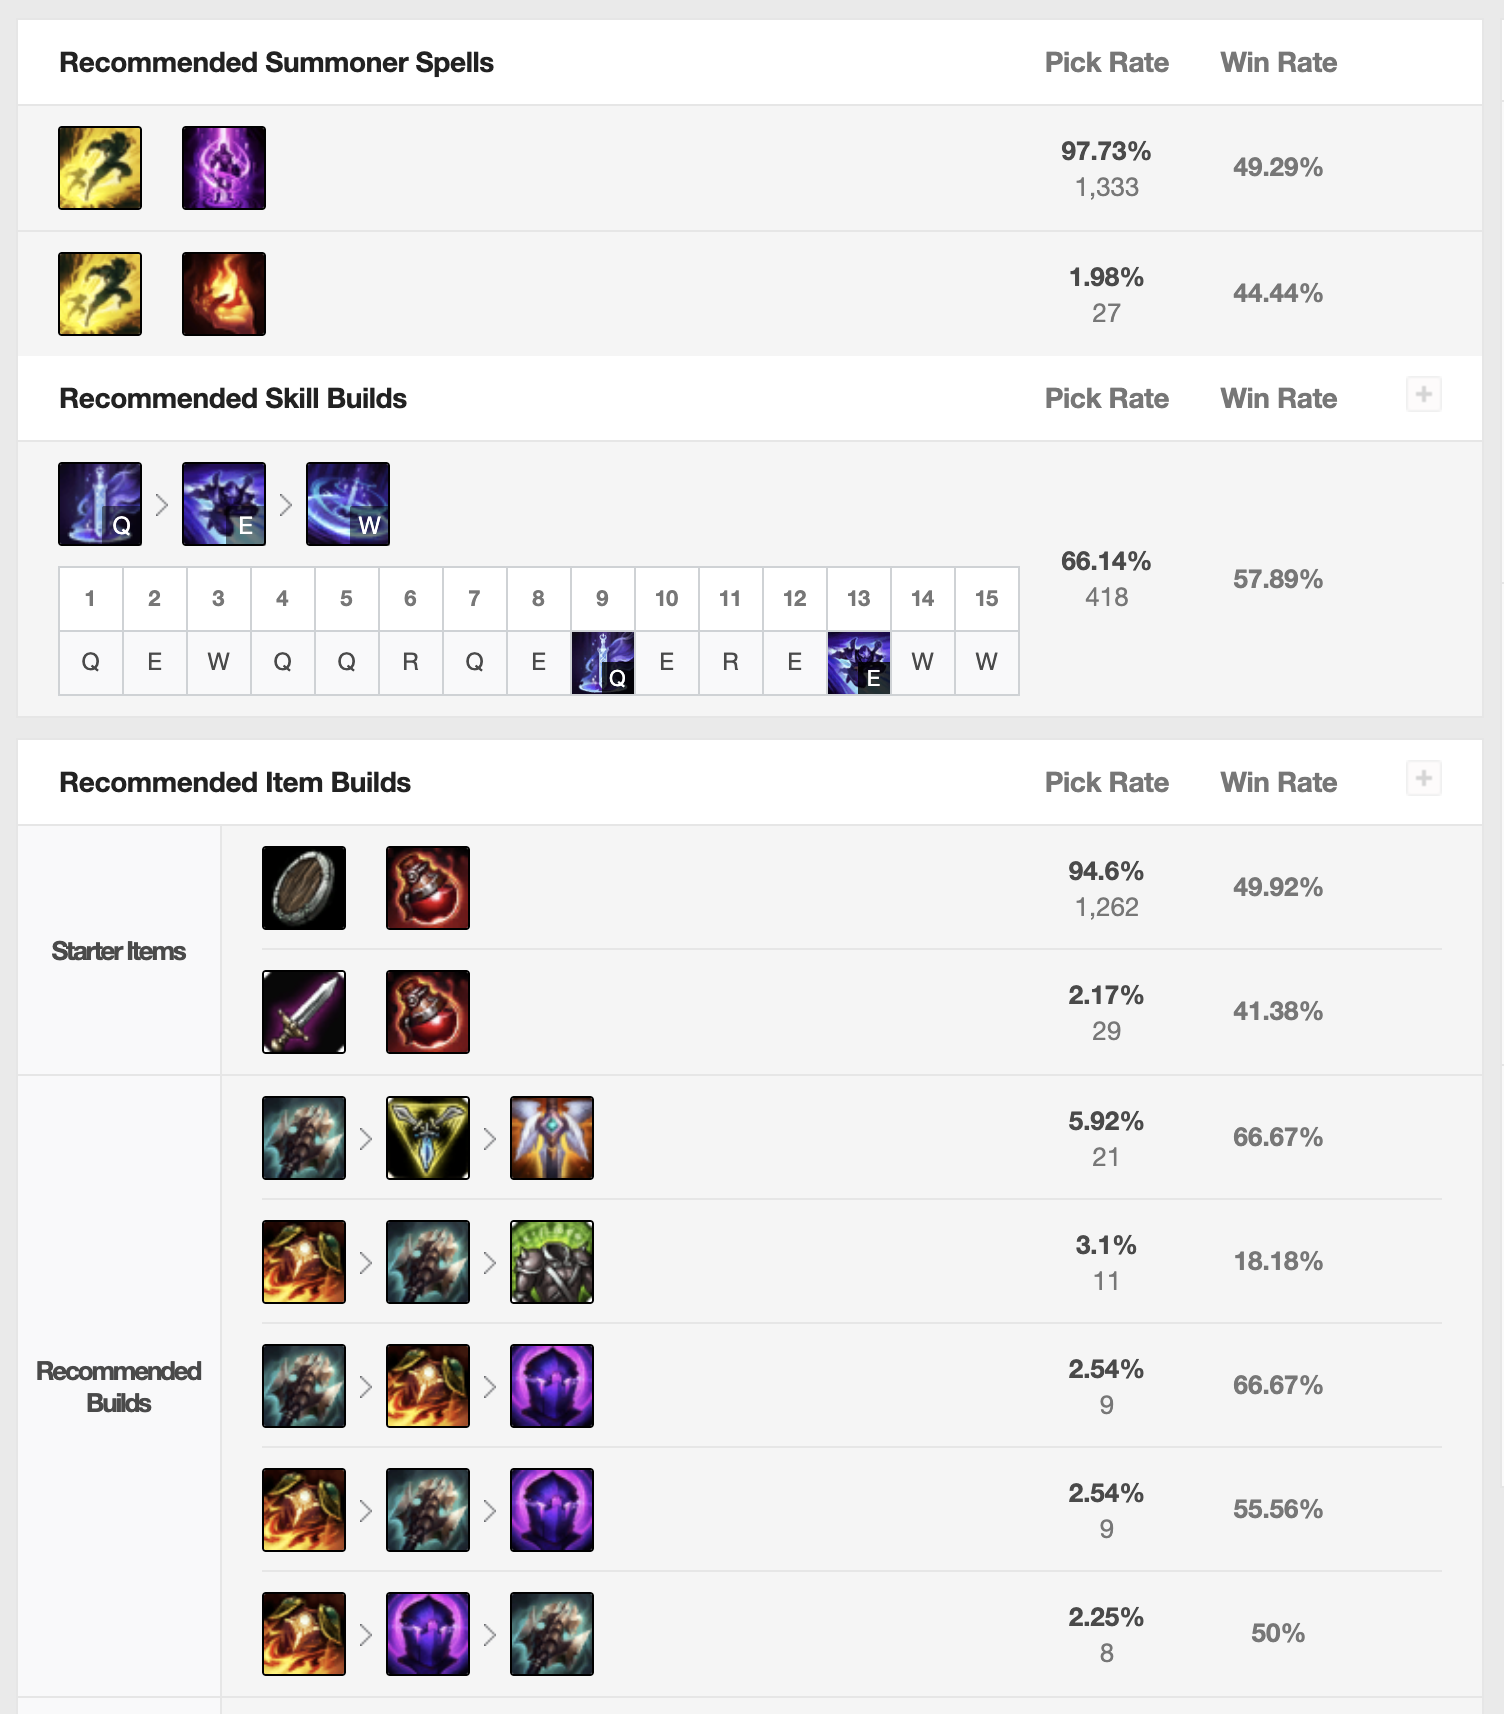
\includegraphics[scale=0.3]{8}
\end{figure}
\begin{figure}[ht]
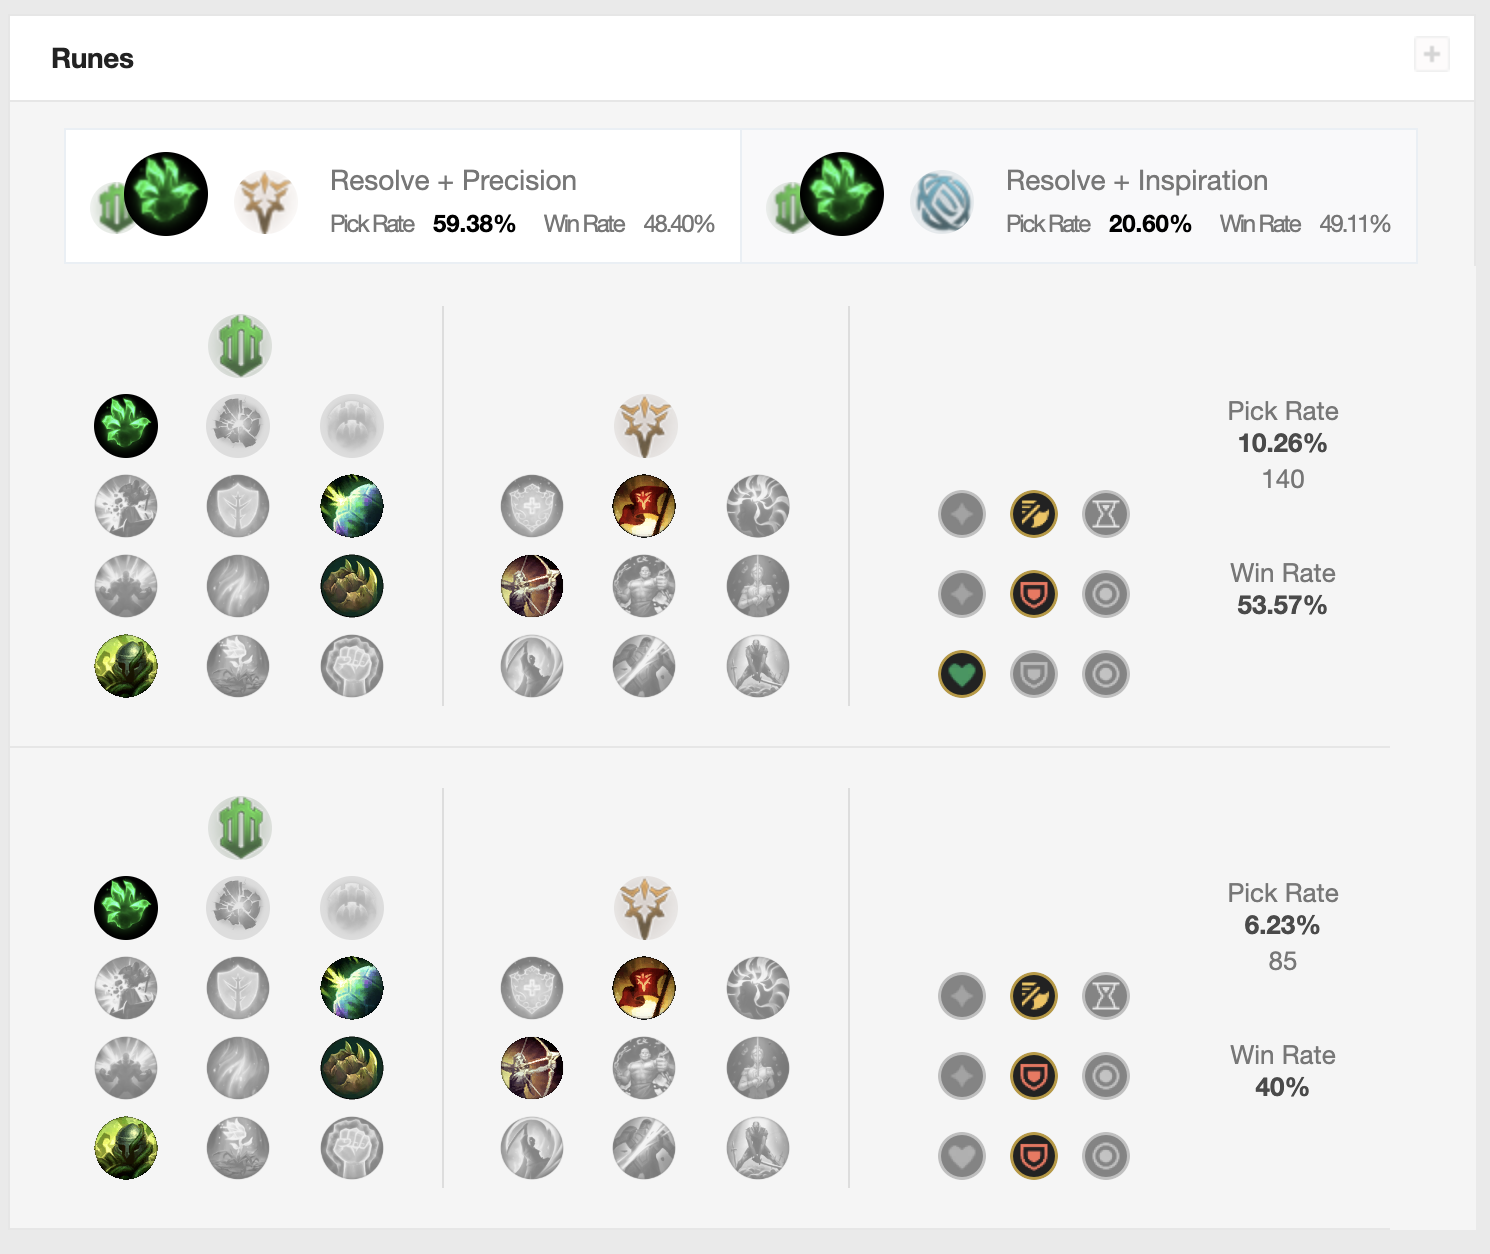
\includegraphics[scale=0.3]{9}
\end{figure}






\end{document}


